\documentclass[tikz,border=4pt]{standalone}
\usetikzlibrary{automata, positioning, arrows.meta}

\tikzset{
  every state/.style = {thick, fill=blue!6, minimum size=10mm},
  >={Stealth[length=2.5mm]},
}

\begin{document}
% A finite automaton that accepts the binary strings ending in 01.
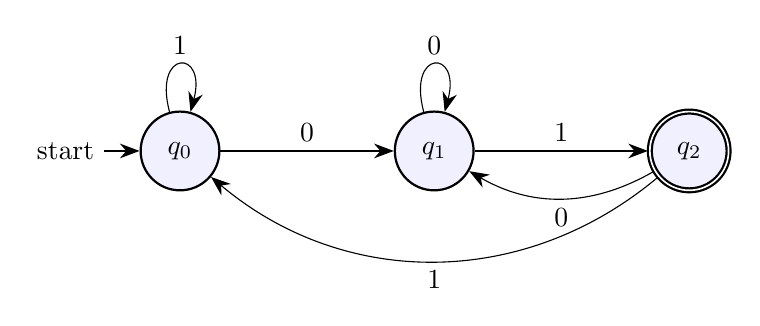
\begin{tikzpicture}[node distance=22mm, auto]
  \node[state, initial]                (q0) {$q_0$};
  \node[state, right=of q0]            (q1) {$q_1$};
  \node[state, accepting, right=of q1] (q2) {$q_2$};

  \draw[->] (q0) to[loop above]   node {1} (q0);
  \draw[->] (q0) --               node {0} (q1);
  \draw[->] (q1) to[loop above]   node {0} (q1);
  \draw[->] (q1) --               node {1} (q2);
  \draw[->] (q2) to[bend left]    node {0} (q1);
  \draw[->] (q2) to[bend left=40] node {1} (q0);
\end{tikzpicture}
\end{document}
